% (find-LATEX "2020-2-C2-fracs-parcs.tex")
% (defun c () (interactive) (find-LATEXsh "lualatex -record 2020-2-C2-fracs-parcs.tex" :end))
% (defun C () (interactive) (find-LATEXsh "lualatex 2020-2-C2-fracs-parcs.tex" "Success!!!"))
% (defun D () (interactive) (find-pdf-page      "~/LATEX/2020-2-C2-fracs-parcs.pdf"))
% (defun d () (interactive) (find-pdftools-page "~/LATEX/2020-2-C2-fracs-parcs.pdf"))
% (defun e () (interactive) (find-LATEX "2020-2-C2-fracs-parcs.tex"))
% (defun o () (interactive) (find-LATEX "2020-2-C2-fracs-parcs.tex"))
% (defun u () (interactive) (find-latex-upload-links "2020-2-C2-fracs-parcs"))
% (defun v () (interactive) (find-2a '(e) '(d)))
% (defun d0 () (interactive) (find-ebuffer "2020-2-C2-fracs-parcs.pdf"))
% (defun cv () (interactive) (C) (ee-kill-this-buffer) (v) (g))
%          (code-eec-LATEX "2020-2-C2-fracs-parcs")
% (find-pdf-page   "~/LATEX/2020-2-C2-fracs-parcs.pdf")
% (find-sh0 "cp -v  ~/LATEX/2020-2-C2-fracs-parcs.pdf /tmp/")
% (find-sh0 "cp -v  ~/LATEX/2020-2-C2-fracs-parcs.pdf /tmp/pen/")
%     (find-xournalpp "/tmp/2020-2-C2-fracs-parcs.pdf")
%   file:///home/edrx/LATEX/2020-2-C2-fracs-parcs.pdf
%               file:///tmp/2020-2-C2-fracs-parcs.pdf
%           file:///tmp/pen/2020-2-C2-fracs-parcs.pdf
% http://angg.twu.net/LATEX/2020-2-C2-fracs-parcs.pdf
% (find-LATEX "2019.mk")
% (find-CN-aula-links "2020-2-C2-fracs-parcs" "2" "c2m202fp" "c2fp")
%
% Video:
% (find-ssr-links "c2m202fp" "2020-2-C2-fracs-parcs" "{nao existe}}")
% (code-video     "c2m202fpvideo" "$S/http/angg.twu.net/eev-videos/2020-2-C2-fracs-parcs.mp4")
% (find-c2m202fpvideo "0:00")

% «.defs»		(to "defs")
% «.title»		(to "title")
% «.deriv-ln»		(to "deriv-ln")
% «.exercicio-1»	(to "exercicio-1")
% «.contas-sem-vai-um»	(to "contas-sem-vai-um")
% «.div-polis»		(to "div-polis")
% «.exercicio-4»	(to "exercicio-4")
% «.together»		(to "together")
% «.P1-2020.1»		(to "P1-2020.1")
%
% «.djvuize»		(to "djvuize")

\documentclass[oneside,12pt]{article}
\usepackage[colorlinks,citecolor=DarkRed,urlcolor=DarkRed]{hyperref} % (find-es "tex" "hyperref")
\usepackage{amsmath}
\usepackage{amsfonts}
\usepackage{amssymb}
\usepackage{pict2e}
\usepackage[x11names,svgnames]{xcolor} % (find-es "tex" "xcolor")
\usepackage{colorweb}                  % (find-es "tex" "colorweb")
%\usepackage{tikz}
%
% (find-dn6 "preamble6.lua" "preamble0")
%\usepackage{proof}   % For derivation trees ("%:" lines)
%\input diagxy        % For 2D diagrams ("%D" lines)
%\xyoption{curve}     % For the ".curve=" feature in 2D diagrams
%
\usepackage{edrx15}               % (find-LATEX "edrx15.sty")
\input edrxaccents.tex            % (find-LATEX "edrxaccents.tex")
\input edrxchars.tex              % (find-LATEX "edrxchars.tex")
\input edrxheadfoot.tex           % (find-LATEX "edrxheadfoot.tex")
\input edrxgac2.tex               % (find-LATEX "edrxgac2.tex")
%
%\usepackage[backend=biber,
%   style=alphabetic]{biblatex}            % (find-es "tex" "biber")
%\addbibresource{catsem-slides.bib}        % (find-LATEX "catsem-slides.bib")
%
% (find-es "tex" "geometry")
\usepackage[a6paper, landscape,
            top=1.5cm, bottom=.25cm, left=1cm, right=1cm, includefoot
           ]{geometry}
%
\begin{document}

%\catcode`\^^J=10
%\directlua{dofile "dednat6load.lua"}  % (find-LATEX "dednat6load.lua")

% %L dofile "edrxtikz.lua"  -- (find-LATEX "edrxtikz.lua")
% %L dofile "edrxpict.lua"  -- (find-LATEX "edrxpict.lua")
% \pu

% «defs»  (to ".defs")
% (find-LATEX "edrx15.sty" "colors-2019")
\long\def\ColorRed   #1{{\color{Red1}#1}}
\long\def\ColorViolet#1{{\color{MagentaVioletLight}#1}}
\long\def\ColorViolet#1{{\color{Violet!50!black}#1}}
\long\def\ColorGreen #1{{\color{SpringDarkHard}#1}}
\long\def\ColorGreen #1{{\color{SpringGreenDark}#1}}
\long\def\ColorGreen #1{{\color{SpringGreen4}#1}}
\long\def\ColorGray  #1{{\color{GrayLight}#1}}
\long\def\ColorGray  #1{{\color{black!30!white}#1}}
\long\def\ColorBrown #1{{\color{Brown}#1}}
\long\def\ColorBrown #1{{\color{brown}#1}}
\long\def\ColorOrange#1{{\color{orange}#1}}

\long\def\ColorShort #1{{\color{SpringGreen4}#1}}
\long\def\ColorLong  #1{{\color{Red1}#1}}

\def\frown{\ensuremath{{=}{(}}}
\def\True {\mathbf{V}}
\def\False{\mathbf{F}}
\def\D    {\displaystyle}

\def\together   {\mathsf{together}}
\def\togetherp#1{\mathsf{together}\left(#1\right)}
\def\apart   {\mathsf{apart}}

\def\drafturl{http://angg.twu.net/LATEX/2020-2-C2.pdf}
\def\drafturl{http://angg.twu.net/2020.2-C2.html}
\def\draftfooter{\tiny \href{\drafturl}{\jobname{}} \ColorBrown{\shorttoday{} \hours}}



%  _____ _ _   _                               
% |_   _(_) |_| | ___   _ __   __ _  __ _  ___ 
%   | | | | __| |/ _ \ | '_ \ / _` |/ _` |/ _ \
%   | | | | |_| |  __/ | |_) | (_| | (_| |  __/
%   |_| |_|\__|_|\___| | .__/ \__,_|\__, |\___|
%                      |_|          |___/      
%
% «title»  (to ".title")
% (c2m202fpp 1 "title")
% (c2m202fp    "title")

\thispagestyle{empty}

\begin{center}

\vspace*{1.2cm}

{\bf \Large Cálculo 2 - 2020.2}

\bsk

Aula nn: frações parciais

\bsk

Eduardo Ochs - RCN/PURO/UFF

\url{http://angg.twu.net/2020.2-C2.html}

\end{center}

\newpage



% (c2m201fracparcp 1 "title")
% (c2m201fracparc    "title")

% «deriv-ln»  (to ".deriv-ln")
% (c2m202fpp 2 "deriv-ln")
% (c2m202fp    "deriv-ln")
% (c2m201fracparcp 2 "2020_deriv_ln.mp4")
% (c2m201fracparc    "2020_deriv_ln.mp4")

Na aula passada nós vimos que $\frac{d}{dx} \ln x = \frac 1x$,

e portanto $\intx{\frac 1x} = \ln x$ \ColorRed{para $x>0$}.

Nós vamos deixar pra ver \ColorRed{depois}

como integrar $\intx{\frac 1x}$ em $x<0$.

\msk

% «exercicio-1»  (to ".exercicio-1")
% (c2m202fpp 2 "exercicio-1")
% (c2m202fp    "exercicio-1")

{\bf Exercício 1.}

\msk

a) $\D \intx{\frac{1}{3x}} = \ColorRed{?}$

\ssk

b) $\D \intx{\frac{1}{3x+4}} = \ColorRed{?}$

\ssk

c) $\D \intx{\frac{2}{3x+4}} = \ColorRed{?}$

\ssk

d) $\D \intx{\frac{a}{bx+c}} = \ColorRed{?}$


\newpage

% «together»  (to ".together")
% (c2m202fpp 3 "together")
% (c2m202fp    "together")
% (find-fline       "~/LATEX/2020-1-C2/20201112_C2_fracoes_parciais_2.pdf")
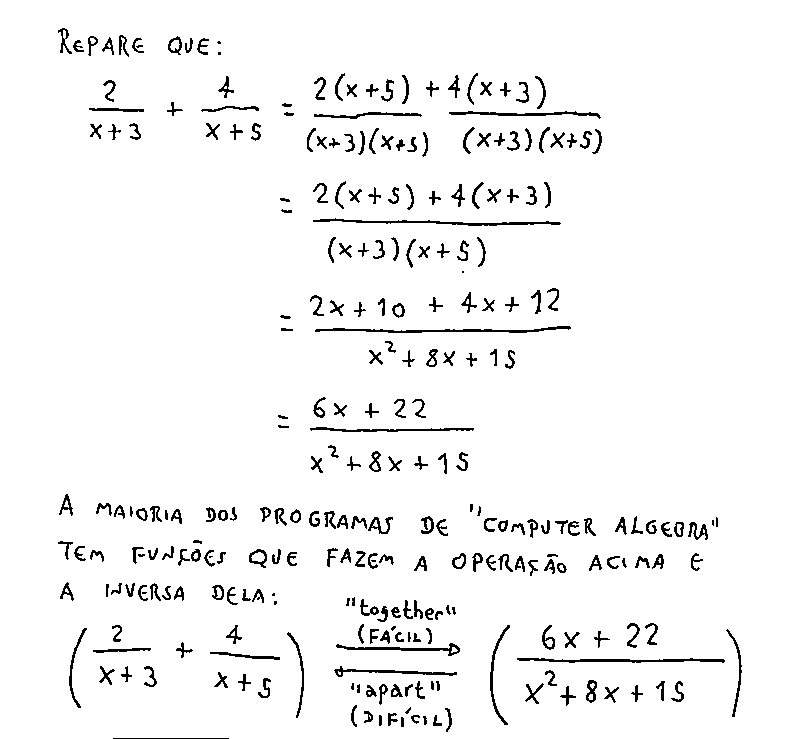
\includegraphics[height=8cm]{2020-1-C2/20201112_C2_fracoes_parciais_2.pdf}

\newpage

{\bf Exercício 2.}

\msk

a) $\D \togetherp{\frac{1}{x+1} + \frac{1}{x-1}} = \ColorRed{?}$ 

\ssk

b) $\D \togetherp{\frac{A}{x-a} + \frac{B}{x-b}} = \ColorRed{?}$ 

\ssk

c) $\D \togetherp{\frac{A}{x-a} + \frac{B}{x-b} + \frac{C}{x-c}} = \ColorRed{?}$ 

% (find-fline "~/LATEX/2020-1-C2/20201112_C2_fracoes_parciais_3.pdf")
%\includegraphics[height=7cm]{2020-1-C2/20201112_C2_fracoes_parciais_3.pdf}



%  (eepitch-vterm)
%  (eepitch-kill)
%  (eepitch-vterm)
% isympy3
% f = 1/(x+1) + 1/(x-1)
% f
% together(f)


\newpage

{\bf Exercício 3.}

% (find-fline "~/LATEX/2020-1-C2/20201112_C2_fracoes_parciais_4.pdf")
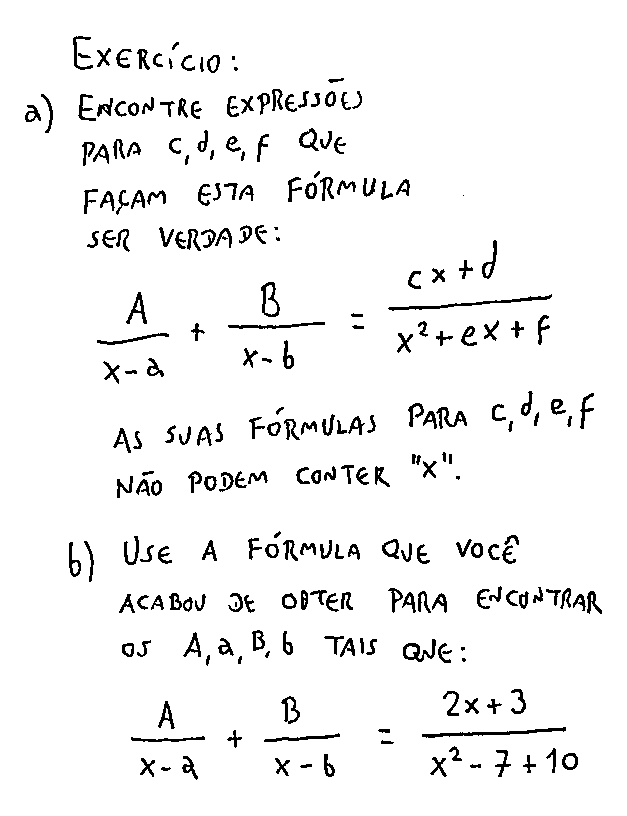
\includegraphics[height=7cm]{2020-1-C2/20201112_C2_fracoes_parciais_4.pdf}

\newpage

% «contas-sem-vai-um»  (to ".contas-sem-vai-um")
% (c2m202fpp 6 "contas-sem-vai-um")
% (c2m202fp    "contas-sem-vai-um")

{\bf Slogan: contas sem ``vai um'' podem ser traduzidas

pra contas com polinômios.}

\ssk

O que mais nos interessa pra Frações Parciais

é \ColorRed{divisão com resto}. Exemplo:

% (find-fline "~/LATEX/2020-1-C2/20201118_C2_div_com_resto_1.pdf")
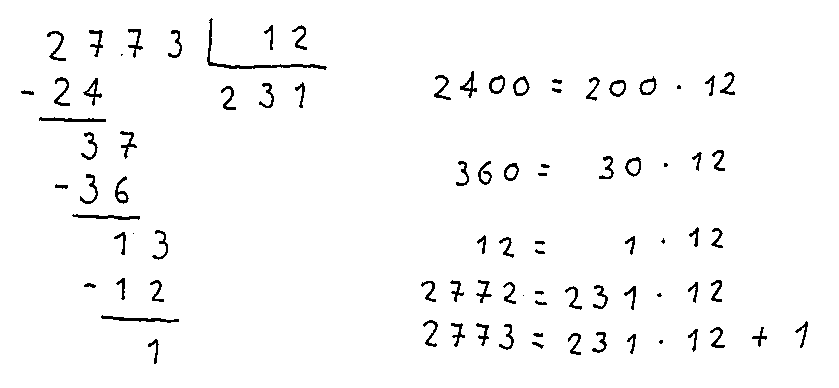
\includegraphics[width=11cm]{2020-1-C2/20201118_C2_div_com_resto_1.pdf}

\newpage

% «div-polis»  (to ".div-polis")
% (c2m202fpp 7 "div-polis")
% (c2m202fp    "div-polis")

...e tradução do exemplo para polinômios:

% (find-fline "~/LATEX/2020-1-C2/20201118_C2_div_com_resto_2.pdf")
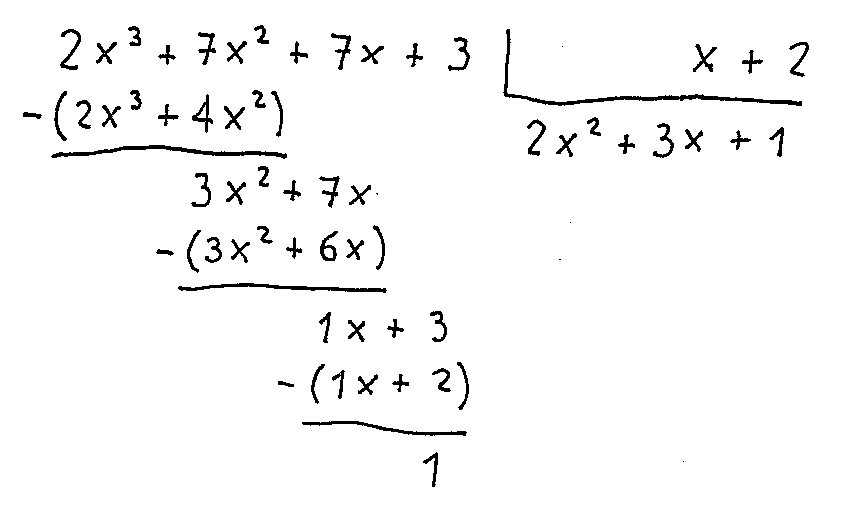
\includegraphics[height=4cm]{2020-1-C2/20201118_C2_div_com_resto_2.pdf}

% (find-fline "~/LATEX/2020-1-C2/20201118_C2_div_com_resto_3.pdf")
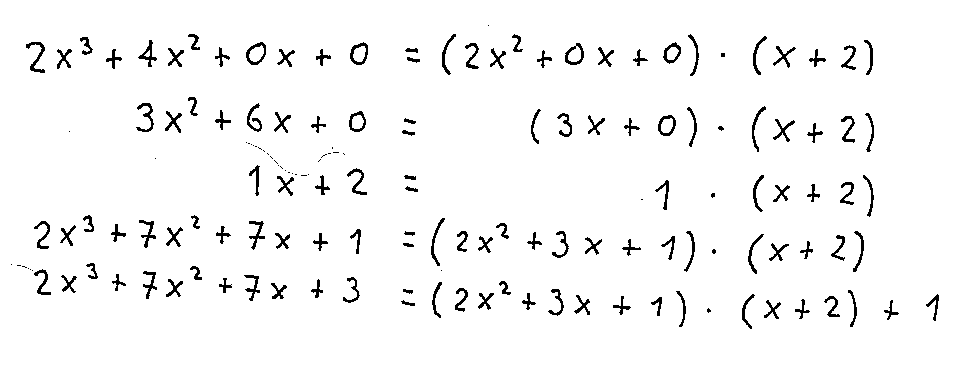
\includegraphics[height=3cm]{2020-1-C2/20201118_C2_div_com_resto_3.pdf}

\newpage

% «exercicio-4»  (to ".exercicio-4")
% (c2m201fracparcp 8 "exercicio-4")
% (c2m201fracparc    "exercicio-4")

{\bf Exercício 4.}

\ssk

Use estas idéias para integrar:

$$\intx{\frac{2x^3 + 7x^2 + 7x + 3}{x+2}} \;\; = \;\; ?$$



\newpage

{\bf Exercício 5.}

\ssk

O que acontece nos casos em que ``teria vai um''?

\ssk

a) Tente fazer a divisão com resto de $x^3$ por $x+2$.

Mais precisamente, encontre um polinômios $R(x)$ e $Q(x)$ tais que

$(x^3) = Q(x) · (x+2) + R(x)$ e $R(x)$ é no máximo de grau 1.

Teste a sua resposta!

\ssk

b) Calcule $\intx{\frac{x^3}{x+2}}$ pelo método acima.

Teste a sua resposta derivando a sua antiderivada para $\frac{x^3}{x+2}$.

\ssk

c) Calcule $\intx{\frac{x^3}{x+2}}$ fazendo a substituição $u=x+2$.

Você deve obter o mesmo resultado que na (b).

\bsk

d) Calcule $\intx{\frac{x^2}{(x+1)(x-1)}}$ por frações parciais.


\newpage

{\bf Dica importante}

\ssk

Lembre que uns dos meus slogans é

``eu só vou corrigir os sinais de igual''...

No slide 7 a igualdade mais importante é a da última linha.

Nós vamos usá-la assim, pra transformar a integral original

em algo fácil de integrar:

\msk

% (find-fline "~/LATEX/2020-1-C2/20201119_C2_div_com_resto_4.pdf")
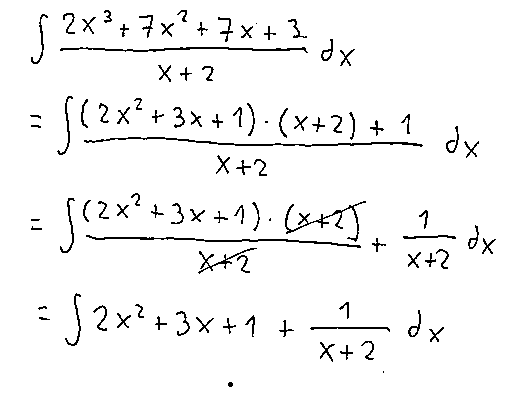
\includegraphics[height=4cm]{2020-1-C2/20201119_C2_div_com_resto_4.pdf}


\newpage

% «P1-2020.1»  (to ".P1-2020.1")
% (c2m202fpp 11 "P1-2020.1")
% (c2m202fp     "P1-2020.1")

{\bf Uma questão da P1 do semestre passado}

A questão 3 da P1 do semestre passado,

\ssk

% http://angg.twu.net/LATEX/2020-1-C2-P1.pdf
\url{http://angg.twu.net/LATEX/2020-1-C2-P1.pdf}

\ssk

era de frações parciais, e eu pus nesse PDF um gabarito

parcial dela, que não inclui nem as contas da divisão de

polinômios nem a verificação de que a nossa integral

está certa. Faça a questão, incluindo a parte que

não está no gabarito.

% (c2m201p1p 5 "questao-3")
% (c2m201p1    "questao-3")





%\printbibliography

\GenericWarning{Success:}{Success!!!}  % Used by `M-x cv'

\end{document}

%  ____  _             _         
% |  _ \(_)_   ___   _(_)_______ 
% | | | | \ \ / / | | | |_  / _ \
% | |_| | |\ V /| |_| | |/ /  __/
% |____// | \_/  \__,_|_/___\___|
%     |__/                       
%
% «djvuize»  (to ".djvuize")
% (find-LATEXgrep "grep --color -nH --null -e djvuize 2020-1*.tex")

 (eepitch-shell)
 (eepitch-kill)
 (eepitch-shell)
# (find-fline "~/2020.2-C2/")
# (find-fline "~/LATEX/2020-2-C2/")
# (find-fline "~/bin/djvuize")

cd /tmp/
for i in *.jpg; do echo f $(basename $i .jpg); done

f () { rm -fv $1.png $1.pdf; djvuize $1.pdf }
f () { rm -fv $1.png $1.pdf; djvuize WHITEBOARDOPTS="-m 1.0" $1.pdf; xpdf $1.pdf }
f () { rm -fv $1.png $1.pdf; djvuize WHITEBOARDOPTS="-m 0.5" $1.pdf; xpdf $1.pdf }
f () { rm -fv $1.png $1.pdf; djvuize WHITEBOARDOPTS="-m 0.25" $1.pdf; xpdf $1.pdf }
f () { cp -fv $1.png $1.pdf       ~/2020.2-C2/
       cp -fv        $1.pdf ~/LATEX/2020-2-C2/
       cat <<%%%
% (find-latexscan-links "C2" "$1")
%%%
}

f 20201213_area_em_funcao_de_theta
f 20201213_area_em_funcao_de_x
f 20201213_area_fatias_pizza



%  __  __       _        
% |  \/  | __ _| | _____ 
% | |\/| |/ _` | |/ / _ \
% | |  | | (_| |   <  __/
% |_|  |_|\__,_|_|\_\___|
%                        
% <make>

 (eepitch-shell)
 (eepitch-kill)
 (eepitch-shell)
# (find-LATEXfile "2019planar-has-1.mk")
make -f 2019.mk STEM=2020-2-C2-fracs-parcs veryclean
make -f 2019.mk STEM=2020-2-C2-fracs-parcs pdf

% Local Variables:
% coding: utf-8-unix
% ee-tla: "c2m202fp"
% End:
